\documentclass[10pt, journal,onecolumn]{IEEEtran}
\usepackage{cite}
\usepackage{graphicx}
\graphicspath{{figure/}}
\usepackage{array}
\usepackage{subfigure}
\usepackage{stfloats}
\usepackage{url}
\usepackage{nicefrac}
\usepackage{amssymb}
\usepackage{amsmath}
%\interdisplaylinepenalty=2500
\usepackage{amsfonts}
\usepackage{amssymb}
\usepackage{relsize}
\usepackage[pdfpagelabels]{hyperref}
\usepackage{float}
\usepackage[round]{natbib}
\usepackage{color}
\usepackage{authblk}
\usepackage{caption}

%\usepackage{kbordermatrix}

\hypersetup{
  colorlinks   = true, %Colours links instead of ugly boxes
  urlcolor     = blue, %Colour for external hyperlinks
  linkcolor    = blue, %Colour of internal links
  citecolor   = blue %Colour of citations
}

\floatstyle{ruled}
\newfloat{algorithm}{tbp}{loa}
\floatname{algorithm}{Algorithm}

\newtheorem{theorem}{Theorem}
\newtheorem{corollary}{Corollary}
\newtheorem{proposition}{Proposition}
\newtheorem{definition}{Definition}
\newtheorem{lemma}{Lemma}

\newcommand{\norm}[1]{\left\lVert#1\right\rVert}
\newcommand{\abs}[1]{\left\lvert#1\right\rvert}
\newcommand{\inner}[1]{\left\langle#1\right\rangle}
\def\b#1{\mathbf{#1}}
\def\t#1{\text{#1}}


\title{Predicting 2014 Ebola Outbreak in West Africa using Network Analysis}

\author{Shafi Bashar, Mike Percy, Romit  Singhai}
\affil{\textit {\{shafiab, mp81, romit\}@stanford.edu}}

\renewcommand\Authands{ and }


\begin{document}

\maketitle

\begin{abstract}
The current Ebola outbreak in West Africa is the worst in history.
Most traditional epidemiological models are compartmental models that have a random-mixing
assumption. These models calculate the
effective reproductive rate of an outbreak. We survey three of these models: the classic
SIR (Susceptible, Infectious, Recovered) model and two extensions used in Ebola research.

In addition to the compartmental models, we discuss a network model that avoids the random-mixing
assumption. This is done by assigning each individual a finite set of permanent contacts.
We also review generated contact network models for SARS, including an urban network, a random network, and
a scale-free network model.
We then describe a world-wide network model that represents traffic flowing across transportation networks.

\end{abstract}




\section{Literature survey}
\label{sec:ReactionPaper}

\subsection{\textbf{The epidemiological SIR model \citep{very_old_paper}}}
\label{SubSec:SIR}

The majority of research in epidemiological theory is based on the compartmental model.
To model the progress of an epidemic in a large population, the
individuals in the population are compartmentalized according to the state of the disease. The most
widely used such model is the SIR model introduced in \citep{very_old_paper}:

\begin{itemize}
\item \textbf{S (Susceptible):} Individuals who have not yet caught the disease from contact with an infectious
  individual.
\item \textbf{I (Infectious):} Individuals who have the disease. They have some probability of
  infecting susceptible people.
\item \textbf{R (Recovered):} Individuals who have experienced the full infectious period, and are
  now non-infectious and immune.
\end{itemize}

The changes among these states over time are represented by a set of differential equations. In
order to capture the dynamics of disease spread over time, a population-wide random mixing model is
assumed, meaning that each individual has a small and equal chance of coming into contact with
any other individual in the population. The basic reproductive number $R_0$
is defined as the average number of secondary cases generated by a primary case in a pool of mostly
susceptible individuals, and is an estimate of epidemic growth at the start of an outbreak if
everyone is susceptible.

\textit{Discussion.} The SIR model is classic and effective, but missing important features
of the Ebola virus: localized spreading behavior, a non-infectious incubation period, and
representation of different methods of transmission.

\subsection{\textbf{The basic reproductive number of Ebola: SEIR model \citep{chowell2004basic}}}

In \citep{chowell2004basic}, the authors model the effect of Ebola outbreaks in Congo 1995 and Uganda
2000 using a compartmental model similar to the SIR model in Section \ref{SubSec:SIR}. However, a
distinct feature of Ebola is that individuals exposed to the virus who become infectious do so
after a mean incubation period. In order to reflect this feature, in \citep{chowell2004basic} the
basic SIR model is modified by adding an additional compartment ``Exposed". The modified SIR model,
i.e. the SEIR model presented in \citep{chowell2004basic} is reproduced in
Figure \ref{fig:SEIR_model}.

\begin{figure}[h!]
\captionsetup{justification=centering}
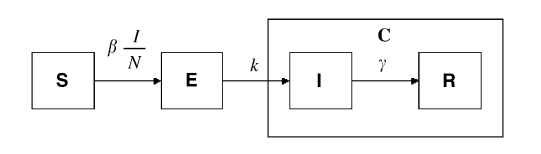
\includegraphics[scale=0.5]{seir_model_fig}
\centering\caption{SEIR model}
\label{fig:SEIR_model}
\end{figure}

In the SEIR model, susceptible (S) individuals in contact with the virus enter the exposed (E) state at a rate of $\beta I / N$. Here,

\begin{eqnarray*}
\beta &=& \text{transmission rate per person per day}\\
N &=& \text{total effective population size}\\
\dfrac{I}{N} &=& \text{probability that contact is made with an infectious individual, assuming uniform random mixing}
\end{eqnarray*}

The exposed (E) individuals undergo an average incubation period of $1/k$ days before progressing to
the infectious (I) state. The exposed state is assumed to be asymptomatic as well as uninfectious.
Infectious (I) individuals move to the R state, either recovered or dead, at a rate of $\gamma$.

The following set of differential equations are used to represent this model:

\begin{eqnarray}
\label{Eq:SEIR}
\dfrac{dS}{dt}	&=&	\dfrac{-\beta SI}{N}\nonumber\\
\dfrac{dE}{dt}	&=&	\dfrac{\beta SI}{N}-kE\nonumber\\
\dfrac{dI}{dt}	&=&	kE-\gamma I\nonumber\\
\dfrac{dR}{dt}	&=&	\gamma I\nonumber\\
C	&=&	kE\nonumber\\
 \end{eqnarray}

Here, $S$, $E$, $I$, and $R$ denote the number of susceptible, exposed, infectious and removed
individuals at time $t$. In the equations, to simplify our notation, we have omitted the dependency
on $t$. $C$ is not an epidemiological state, however is useful to keep track of the cumulative
number of cases from the time of the onset of the outbreak.

In order to model the effect of intervention on the spread of the disease, in the above model, the
transmission rate $\beta$ is modeled as a function of time. At the initial phase of the outbreak,
before intervention, $\beta$ is parameterized by $\beta_0$. After intervention, the value of
$\beta$ transitions from $\beta_0$ to $\beta_1$, $\beta_0>\beta_1$ as follows:

\[
\beta(t)=\begin{cases}
\beta_{0} & t<\tau\\
\beta_{1}+(\beta_{0}-\beta_{1})\exp\left(-q\left(t-\tau\right)\right) & t\ge\tau
\end{cases}
\]

Where $\tau$ is the time when interventions begin and $q$ controls how quickly the rate
of transmission changes from $\beta_0$ to $\beta_1$.

The Ebola data for the 1995 Congo and 2000 Uganda outbreaks were represented as $(t_i,y_i)$,
$i=1,2,\ldots,n$ where $t_i$ represents $i$th reporting time and $y_i$ the cumulative number of
infectious cases from the beginning of the outbreak of to time $t_i$.  The model parameters
$\Theta=(\beta_0,\beta_1,k,q,\gamma)$ were estimated using a least-square fit by fitting these data to
the cumulative number of cases $C(t,\Theta)$ in Equation \ref{Eq:SEIR}. The initial condition and
appropriate of range of the parameters were taken from Empirical studies, e.g. an incubation period
between $1$ and $21$ days and infectious period between $3.5$ and $10.7$ days were assumed. Once the
parameters are estimated, the basic reproductive number was calculated using the following formula:

\begin{equation}
R_0 = \dfrac{\beta_0}{\gamma}
\end{equation}


In addition to calculating $R_0$, \citep{chowell2004basic} also proposed an analogous continuous time Markov chain model based on the estimated parameters. The transition rates were defined as follows:

\begin{center}
\begin{tabular}{|c|c|c|}
\hline
Event & Effect & Transition Rate\tabularnewline
\hline
\hline
Exposure & (S,E,I,R)$\to$(S-1,E+1,I,R) & $\beta SI/N$\tabularnewline
\hline
Infection & (S,E,I,R)$\to$(S,E-1,I+1,R) & $kE$\tabularnewline
\hline
Removal & (S,E,I,R)$\to$(S,E,I-1,R+1) & $\gamma I$\tabularnewline
\hline
\end{tabular}
\end{center}

The event times $0<T_1<T_2<\ldots$ at which an individual moves from one state to another are modeled as a renewal process with increments distributed exponentially,

\begin{equation}
P(T_k-T_{k-1} > t | T_j, j\leq k-1) = \exp(-t \mu (T_{k-1}) )
\end{equation}

Here,
\[
\mu (T_{k-1}) = \frac{1}{\dfrac{\beta(T_{k-1}) S(T_{k-1}) I(T_{k-1})}{N} + k E(T_{k-1}) + \gamma I(T_{k-1})}
\]

Based on the above stochastic model, \citep{chowell2004basic} provides the results of a Monte Carlo
simulation that shows good agreement with the actual data.

\textit{Discussion.} While the SEIR model adds needed features to the SIR model, it still suffers
from the random mixing assumption and only represents a single infectious state.

\subsection{\textbf{Understanding the dynamics of Ebola epidemics: SEIHFR model \citep{legrand2007understanding}}}

Similar to \citep{chowell2004basic}, \citep{legrand2007understanding} also studies the Ebola
outbreaks in Congo in 1995 and Uganda in 2000. However, a major difference from
\citep{chowell2004basic} is that \citep{legrand2007understanding} modeled the spreading of disease
in heterogeneous settings. In order to gain better insight of the epidemic dynamics,
\citep{legrand2007understanding} subdivided the infectious phase into three stages:

\begin{itemize}
\item Transmission of infection in community setting (I)
\item Transmission of infection in hospital setting (H)
\item Transmission of infection after death assuming a traditional funeral (F)
\end{itemize}


The SEIHFR compartmental model is reproduced in Figure \ref{fig:SEIHFR_model}, with transition rates
following:

\begin{figure}[h!]
\centering
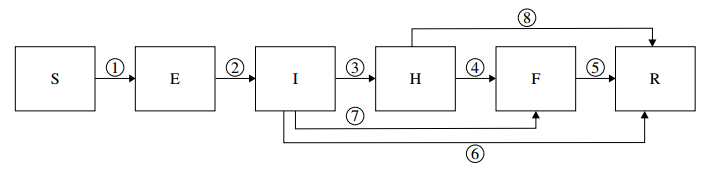
\includegraphics[scale=0.5]{seihfr_model_fig}
\caption{SEIHFR model}
\label{fig:SEIHFR_model}
\end{figure}

\begin{center}
\begin{tabular}{|c|c|c|}
\hline 
Transition $(i)$ & Effect & Transition Rate $(\lambda_i)$ \tabularnewline
\hline 
\hline 
1 & (S,E)$\to$(S-1,E+1) & $(\beta_{I}SI+\beta_{H}SH+\beta_{F}SF)/N$\tabularnewline
\hline 
2 & (E,I)$\to$(E-1,I+1) & $\alpha E$\tabularnewline
\hline 
3 & (I,H)$\to$(I-1,H+1) & $\gamma_{h}\theta_{1}I$\tabularnewline
\hline 
4 & (H,F)$\to$(H-1,F+1) & $\gamma_{dh}\delta_{2}H$\tabularnewline
\hline 
5 & (F,R)$\to$(F-1,R+1) & $\gamma_{f}F$\tabularnewline
\hline 
6 & (I,R)$\to$(I-1,R+1) & $\gamma_{i}(1-\theta)(1-\delta_{1})I$\tabularnewline
\hline 
7 & (I,F)$\to$(I-1,F+1) & $\delta_{1}(1-\theta_{1})\gamma_{d}I$\tabularnewline
\hline 
8 & (H,R)$\to$(H-1,R+1) & $\gamma_{ih}(1-\delta_{2})H$\tabularnewline
\hline 
\end{tabular}
\end{center}

Where the model parameters are as follows: $ \beta_I, \beta_H, \beta_F$ are the transmission
coefficients in community, hospital and funeral settings, $\theta_1$ is the fraction of infectious
cases hospitalized, $\delta_1$ is the fatality ratio of infectious people, $\delta_2$ is the
fatality ratio of hospitalized patients, $\delta_1$ and $\delta_2$ are computed such that overall
fatality ratio is $\delta$, $1/\alpha$ is the mean duration of the incubation period, $1/\gamma_h$
is the mean duration from symptom onset to hospitalization, $1/\gamma_{i}$ is the mean duration of
the infectious period for survivors, $1/\gamma_{d}$ is the mean duration of the infectious period
before death, $1/\gamma_{dh}$ is the mean duration from hospitalization to death, $1/\gamma_{ih}$ is
the mean duration from hospitalization to the end of infectiousness for survivors, and
$1/\gamma_{f}$ is the mean duration from death to burial.

In order to model the effect of interventions, a two step approach is used:

\begin{itemize}
\item Before intervention, population was exposed to the cases in community, hospitalization as well as funeral
\item After intervention, no transmission occurred at hospital or funeral, i.e. $\beta_H = \beta_F = 0$. The transmission coefficient in the community is decreased by a factor of $(1-z)$.
\end{itemize}

In the above mentioned model, parameters $(\beta_I, \beta_H, \beta_F , z)$ were estimated by fitting
the model to the morbidity data from the 1995 Congo and 2000 Uganda outbreaks using approximate maximum
likelihood. The estimates of other parameters in the above model were drawn from prior work.

Simulations of the stochastic model were performed using Gillespie's first reaction method \citep{gillespie1976general}. At each iteration of the algorithm, a time $\tau_i$ is drawn from an exponential distribution with parameter $\lambda_i$ for each of the transition. Here, $\lambda_i$ is the transition rate of the transition $i$. The next transition $\mu$ is the transition that has the minimum time to occurrence ($\tau_\mu$). Counts in each compartment are updated accordingly. In addition to the simulation result,  \citep{legrand2007understanding} also presented the basic reproductive rate as a function of $(\beta_I,\beta_H,\beta_F,\gamma_h,\gamma_{dh},\gamma_{ih},\gamma_d,\theta_1,\delta_1,\delta_2)$.

\textit{Discussion.} The SEIHFR model comes even closer to modeling the real-life behavior of Ebola,
but due to being a compartmental model continues to suffer from the random mixing assumption.
Additionally, as more states are added to the compartmental model, complexity increases and ease of
characterizing and understanding the model is diminished.

\subsection{\textbf{Discussion: SIR \citep{chowell2004basic, legrand2007understanding} vs. networks \citep{newman2002spread}}}

\citep{chowell2004basic, legrand2007understanding}, as described in previous sections, modeled the spread of Ebola using the
compartmental modeling procedure. Even though \citep{legrand2007understanding} modified the
SEIR model to reflect the heterogeneity of infection states, the underlying assumption is still
random mixing. A disease like Ebola spreads via networks formed by physical contact among individuals.
While an individual may have the same number of contacts per unit
time in either a random mixing model or a network contact model, within a static network model the set of
contacts is fixed, versus a random-mixing model wherein it is continually changing.
A static network model thus captures the permanence of many human relationships.

In \citep{newman2002spread}, the authors extend the concept of the SIR model in network analysis.
They provide an exact solution to the SIR model of epidemic disease on networks of various kinds.
This is achieved using a combination of mapping to percolation models and using edge probability generating functions.

Transmissibility $T$ of a disease is defined as the average probability that an infectious
individual will transmit the disease to a susceptible individual with whom they have contact.
The epidemic threshold $T_c$ is the minimum transmissibility required for an outbreak to become
a large-scale epidemic. The authors provide the relation between the basic reproductive number
$R_0$ of an SIR network and the transmissibility $T$ as follows:
\[
R_0 = T  \dfrac{\left\langle k^2 \right\rangle}{\left\langle k \right\rangle-1}
\]

In addition, \citep{newman2002spread} also provide the value of epidemic threshold $T_c$.  In an uncorrelated network, it is given by:

\[
T_c =\dfrac{\left\langle k \right\rangle}{\left\langle k^2 \right\rangle - \left\langle k \right\rangle}
\]

Here, $\left\langle k \right\rangle$ and $\left\langle k^2 \right\rangle$ are the mean degree and
mean square degree of the network. Parameters for Poisson and power law networks are chosen such
that all three networks share the same epidemic threshold. The authors predict average size
of the outbreak $\left\langle s \right\rangle$ and the probability of an epidemic $S$.

The results in \citep{newman2002spread} allow us to compare more directly the relationships between
random mixing models and network models under certain assumptions. This may prove handy in
validating our models.


\subsection{\textbf{Contact Networks for Epidemiology \citep{meyers2005network}}}

In our search for existing literature on the use of contact networks to model the spread of Ebola, we haven't come
across any previous work that precisely does this, possibly due to the lack of detailed data in the
locations historically affected by the disease.
In \citep{meyers2005network}, the authors model the spread of the 2002-2003
outbreak of SARS in Hong Kong and Canada using a network model. A contact network model attempts to
characterize every interpersonal contact that can potentially lead to disease transmission in the
community. Each person in the community is represented as a node in the network and each contact between
two people is represented as an edge connecting them.
In \citep{meyers2005network}, the authors presented three different contact network models for SARS:

\begin{itemize}
\item \textbf{Urban Network:} A plausible contact network for an urban setting was generated using
  computer simulation based on the data for the city of Vancouver. $N=1000$
  households were chosen at random from Vancouver household size distribution statistics yielding
  approximately 2600 people. Household members were given ages based on age distribution
  statistics and assigned to schools, occupations, hospitals as patients, and caregivers according
  to statistics from public data.
\item \textbf{Random Network:} The above urban networks offers high degree of realism, however is quite complex. In
  addition to the urban model, a random network with Poisson degree distribution in which
  individuals connect to others independently and uniformly at random.
\item \textbf{Scale-free Network:} There may be individuals in the network called ``superspreaders''
  with unusually large numbers of contacts or ``supershedders" who are unusually effective at
  excreting the virus into the environment they share with others. Neither the urban nor the random
  networks contains significant number of superspreaders. To incorporate the effects of
  superspreader in disease transmission, \citep{meyers2005network} also studies a network with
  truncated power law degree distribution. This type of network has a heavy tail of superspreaders.
  These individuals despite being few in numbers had a profound effect on the outbreak patterns.
\end{itemize}

\textit{Discussion.} \citep{meyers2005network} extended the result from \citep{newman2002spread} to calculate the fate
of an outbreak based on its initial condition, the probability that a patient zero with degree $k$ will
start an epidemic, and the probability that an outbreak of size $N$ will start an epidemic. However,
\citep{newman2002spread} did not capture the temporal progression of the epidemic, instead
providing an overall number and distribution of the infected individuals.
The authors predicted the probability $S$
that an outbreak with $R_0>1$ will lead to an epidemic for their three networks. $S$ is often
significantly less than $1$ and can be different for two networks with the same $R_0$. Outbreaks
are consistently less likely to reach epidemic proportions in power law networks than in
the others. $R_0$ is a valuable epidemiological quantity, however it has its limit since $R_0$ is
a function of both the transmissibility of a disease and the contact patterns that underlie the
transmission. Therefore, measuring $R_0$ in a location where contact rates are unusually high will
lead to an estimate that is not appropriate for the larger community. Estimating $T$ instead of
$R_0$ may give us a way out of this difficulty.


\subsection{\textbf{Report assessing the international spreading risk of Ebola \citep{gomes2014assessing}}}

A recent study \citep{gomes2014assessing} gathered data from the Disease Outbreaks News of
the WHO and used what they call the Global Epidemic and Mobility Model to predict the spread of the
current (2014) Ebola outbreak. In this model, the world is divided into geographcal regions defining a
subpopulation network, modeling connections among subpopulations representing traffic flows due to
transportation infrastructure.

Like \citep{legrand2007understanding}, they use the SEIHFR compartmental disease model and compare
it with the more traditional SEIR model, while simulating
an ensemble of possible epidemic evolutions for observables such as newly-generated
cases, time of arrival of infection, and the number of traveling disease carriers.
The parameter $\theta_1$ is computed so that $\theta\%$ of infectious cases
are hospitalized.

The expression for the basic reproductive number $R_0$ is obtained using the sum of three terms
for this model:

$$
R_0 = R_I + R_H + R_F
$$

Where $R_I$ is a term that accounts for transmissions in the community, $R_H$ accounts for
transmissions in the hospital, and $R_F$ accounts for infections due to dead individuals.
Parameters were fit using latin hypercube sampling of the parameter space defined by the
vector $P = (R_I, R_H, R_F)$.

To make predictions, the authors ran Monte Carlo simulations exploring the value of $R_0$ while relying on results reported
in \citep{legrand2007understanding} and elsewhere for the rest of the model parameters.

\textit{Discussion.} The approach used in \citep{legrand2007understanding} appears to be the state of the art in epidemic prediction for
situations where the available data is very limited. Unfortunately, as previously discussed, the
SEIHFR model has a random mixing assumption that does not reflect reality over large areas.
It may be possible to use small world networks or other generated networks to model locality
more effectively based on population density and geographical information.


%%%%%%%%%%%%%%%%%%%%%%%%%%%%%%%%

\section{Project Proposal}
\label{sec:ProjectProposal}

\subsection{Data set}

The data set we plan to use \citep{cmriversdata} is an aggregation of Ebola outbreak data
from multiple sources, including the WHO, the Liberia Ministry of Health, and the Sierra Leone
Ministry of Health. The data set consists of time series totals for suspected infected, confirmed
infected, and dead on an almost-daily basis across several countries, and counties within countries.
To model a world-wide contact network, we will be using information from additional sources, such
as the CIA factbook or World Trade Organization (WTO) economic trade data between countries.



\subsection{Project plan}


\begin{enumerate}

\item \textbf{Estimating model parameters and basic reproduction number for 2014 Ebola data using a random mixing model:}
  In the first phase of the project, we are planning to use the SEIR model proposed in
  \citep{chowell2004basic} as a baseline model, and estimate the model parameters $\beta_0, \beta_1,
  k, q, \gamma$  and basic reproduction number $R_0$ to fit the data obtained from current Ebola
  outbreak. Once the parameters are obtained, we are planning to use these parameters to perform
  prediction of the epidemic assuming a fully mixed model. To benchmark our prediction, we are
  planning to use the prediction performed by the CDC \citep{meltzer2014estimating}. We are
  interested in observing how different parameters in the model affect the spread of the disease. To
  this end, we are planning to vary critical parameter values, such as mean incubation period and
  transmission rate, in order to observe their effects on disease growth.

\item \textbf{From random mixing model to contact network:} \citep{newman2002spread,
  meyers2005network} extended the basic SIR model to network analysis. Whether this model is readily
  applicable to the modified (SEIR, SEIHFR) compartmental models used previously in Ebola research
  \citep{chowell2004basic, legrand2007understanding} is not immediately clear. In the second phase of
  our project, we will model contact networks using the basic reproductive numbers and other
  parameters obtained in phase 1. We will then estimate the propagation of disease on these
  contact networks by assuming an initial number of infected nodes. Since, in a contact network based
  model, each node can propagate the disease to only its immediate contacts, i.e. the neighboring
  nodes, the spreading of disease in a contact network based model will be different from our first
  phase of analysis, in which a random mixing paradigm is assumed. \\

  In the case of the currently-affected African countries, such as Liberia,
  we have county-level data points, and are planning to use that county-level data in different ways.
  One approach is to model individuals as nodes in a small-world network, and
  since the individuals within a particular county are more likely to have contact with each other,
  we may use a different probability of adding long-range links within a county than between counties.
  Another approach is to model each county as a node in a wide-area ``internetwork''.
  In any case, the number of edges between different counties can be dependent on different
  demographic parameters such as the underlying transportation networks, distance between counties,
  or amount of trade between the regions.
  Within each county, we also plan to simulate disease-spread behavior using different types of
  generated contact networks, including random graphs, small world networks, and scale-free
  networks. \\

  Thus far, the growth curve of the Ebola virus in Liberia has been exponential, while in other
  places like Guinea and Sierra Leone the growth curve is more linear \citep{cmriversdata}.
  When using a compartmental model for analysis, we will model different values of
  $R_0$.
  When modeling as a contact network, we can start by calculating a single value of transmissibility
  $T$ and model contact networks for Liberia or Guinea differently using different average degrees of
  nodes.
  We can also try using different types of network models for different places
  and observe the effect of these different assumptions on the spread of the disease. \\

\item \textbf{Possibility of Ebola becoming a world-wide epidemic:} In \citep{gomes2014assessing},
  the authors use airport network data to predict the spread of Ebola to different parts of the
  world. In the third phase of our project, we are planning to use a similar approach to predict the
  spread of the epidemic over a wider region of the world. To this end, we will make use of the estimation
  parameters and insight gained in phase 1 and phase 2 of our project. In order for the disease to
  spread, we need to consider the underlying contact networks between different regions of the
  world. In order to model such a contact network, we can make use of public data such
  as transportation networks, trade routes, and levels of trade between countries and regions.
  We may even be able to use demographic information.
  Since traditional funeral practices in certain regions may increase
  the chance of spreading the diease, such as setting the dead afloat in a river, we can also make
  use of river flow data.

\end{enumerate}



%\begin{figure}[!ht]
%\centering
%\subfigure[]{
%\includegraphics[scale=0.42]{fig3a}
%\label{fig:subfig1_bpsk}}
%\subfigure[]{
%\includegraphics[scale=0.42]{fig3b}
%\l.abel{fig:subfig2_bpsk}}
%\subfigure[]{
%\includegraphics[scale=0.42]{fig3c}
%\label{fig:subfig3_bpsk}}
%\subfigure[]{
%\includegraphics[scale=0.42]{fig3d}
%\label{fig:subfig4_bpsk}}
%\caption[]{MMSE difference function $f_D(p,a)$ for different values of $a = e_i^2 \diagup b_i^2$ for (a) BPSK (b) QPSK (c) 16-QAM (d) 64-QAM.}
%\label{fig:mmseD_bpsk}
%\end{figure}
%


%%%%%%%%%%%%%%%%%%%%%%%%%%%%%%%%%%%%%%%%%%%
%\appendices
%\section{Proof of Proposition \ref{thm:secrecy}}


\bibliographystyle{plainnat}
\bibliography{bib_ref}


\end{document}
